% !TEX root = report.tex

\chapter{Bot Architecture}
\label{chap:implementation}

This chapter will describe the overall structure of \massexpand and its major components.

\section{Overall Structure}

The starting point of the creation of the bot was the example AI bot distributed with BWAPI. The example bot contains a main update loop and all event listeners BWAPI supports. It also provides some sample code for giving orders to units. We left the example module mostly intact for future reference. We added calls to methods of a new class, HighCommand, which would be the entry point for our code. Leaving the example code intact meant we could easily update BWAPI including the example bot. To use our code, we would only have to add the calls to HighCommand back to the example code.

In our first attempts to create a bot, we tried using BWSAL, which is described in section~\ref{sec:bwsal}. We quickly abandoned BWSAL after realizing it would be hard to adapt it to our ideas. What we kept from BWSAL were two helper classes, UnitGroup (an excellent class to select and divide groups of units) and BuildingPlacer (a class with methods to determine where a building should be built). We also kept the the naming convention used by BWSAL (the "managers").

The managers are all responsible for a part of the bot's operation. For example, we have a manager keeping track of our minerals and gas, a manager storing information about enemy units and a manager overseeing construction of buildings and units. Organizing the bot this way allows us to separate code responsible different areas of the bot operation, and also allows us to structure the way the information obtained from the game flows through our bot, resulting in commands sent back to the game. This flow of information is shown in Figure~\ref{fig:flowofinformation}.

\begin{figure}[htb]
\centering
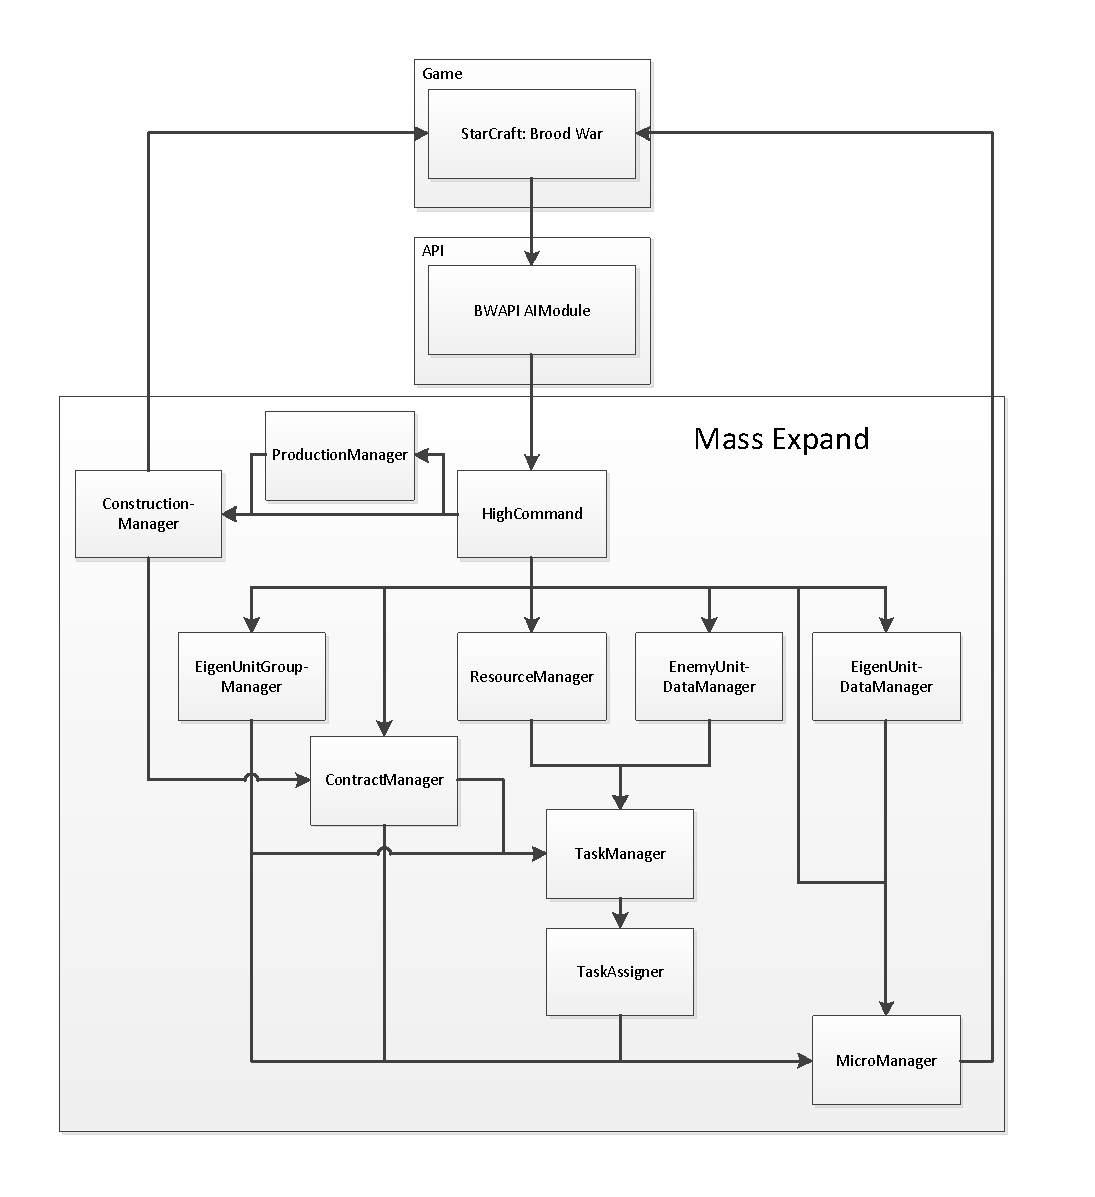
\includegraphics[width=\textwidth, trim= 0mm 10mm 0mm 10mm, clip]{images/flowofinformation}
\caption{The flow of information from StarCraft through Mass Expand to Micro\-Manager and Construction\-Manager, which send commands back to StarCraft.}
\label{fig:flowofinformation}
\end{figure}

Figure~\ref{fig:flowofinformation} can also be seen as a parallelized version of the main loop of our bot. However, in practice, the managers are called in serial form, in a specific order. When the main loop of HighCommand is run, the managers are called in the following order:

\begin{description}
\item[EigenUnitDataManager] Data about our own units is updated.
\item[EigenUnitGroupManager] Any new units we have are assigned to groups, and the groups are balanced.
\item[EnemyUnitDataManager] Data about visible enemy units is updated, such as their position and health.
\item[ResourceManager] Lists of mineable gas and mineral deposits close to our bases are updated.
\item[ProductionManager] Plans are made for the construction of buildings, units, upgrades and technology.
\item[ConstructionManager] Plans made by ProductionManager are executed if possible.
\item[ContractManager] Build orders for buildings are delegated to drones and a suitable build location is found for them.
\item[TaskManager] Tasks are collected from the other managers.
\item[TaskAssigner] The collected tasks are assigned to units and unitgroups.
\item[MicroManager] Mobile units are given specific movement instructions, based on their tasks and enemies near their location.
\end{description}

The managers can be roughly divided into three groups: observation (Eigen\-Unit\-Data\-Manager, Eigen\-Unit\-Group\-Manager, Enemy\-Unit\-Data\-Manager), planning (Resource\-Manager, Production\-Manager, Construction\-Manager, Contract\-Manager), and action (Task\-Manager, Task\-Assigner, Micro\-Manager). First, we see what units we have, and what units the enemy has (observation). Next, we check what we should build, considering the units we have and the enemy has (planning). Finally, we give orders to our units, reacting to the current game state (action). The actions result in a new game state, which will be observed at the next iteration of the game loop.

HighCommand and the managers will be described in more detail in the following sections.

\section{HighCommand}

HighCommand is the control center of our bot. It does three things:

\begin{itemize}
\item It instantiates the managers and calls them in the right order.
\item It listens for game events from BWAPI and forwards them to the right managers.
\item It draws extra textual and graphical information on top of the game interface for debugging purposes.
\end{itemize}

The specific order in which HighCommand calls the managers is listed in the previous section. The order is important because some managers require updated information from other managers to function.

BWAPI allows bots to draw extra information on the screen, on top of the game interface. This is a handy feature to show internal information of the bot that would otherwise be invisble. HighCommand displays the location and type of tasks, the assignment of units to tasks (shown as lines from units to tasks), the build queue and current contracts (drones that are ordered to build a structure).

\section{EigenUnitDataManager}

EigenUnitDataManager records data about our own units. BWAPI provides many methods to get data about our own units, but this data might change each call of the main loop. BWAPI allows bots to update each frame of the game, at a rate of 25 frames per second. By recording data from the last frame, we are able to detect changes. One of such changes we monitored for was a loss of hit points, which indicated a unit was being attacked (a later version of BWAPI added a function to detect whether a unit was under attack). Another option this manager provides is to record which of our units were seen by the enemy and where and when this occured. If one of our units ever moved within visual range of an enemy unit, we can assume the enemy knows about that unit and will act on that information.

\section{EigenUnitGroupManager}

This manager divides all our mobile units into persistent groups. Such groups can be manipulated as if they were a single unit: orders given to a unitgroup are passed to all the units in the group. Unitgroups are implemented in the UnitGroup class from BWSAL, which provides many helpful selector functions. With these functions, we can for example easily "get all flying units in this group". The selector functions can be chained, allowing us to manage our units with very concise code.

The groups that the EigenUnitGroupManager maintains are updated whenever the number of units we have changes. When a new unit is created, it is either assigned to an existing group or given its own new group. When one of our units dies or we otherwise lose control of it, it is removed from its group. The groups are then balanced by reassigning units between groups, according to various rules.

For example, new Overlords are always given a new group of their own. However, if there is a group of Mutalisks that does not have any Overlords, the Overlord will be moved to the Mutalisk group in the balancing step. It is good practice to have a Overlord with Mutalisks (both flying units) because the Overlord can detect stealth units, which are then easily taken out by the Mutalisks.

Drones are a special case. We keep all Drones in a single group. While they are capable of combat, they are best used for gathering resources and construction of buildings. By keeping them in a special group we make sure they are not accidentally assigned to combat tasks.

\section{EnemyUnitDataManager}

EnemyUnitDataManager keeps track of enemy units. By default, BWAPI only allows bots access to visible units. However, we we want to retain information about them when they become invisible, such as when they use a stealth ability or move into fog of war. Units can also transform into a different unittype. In that case, we need to make sure we recognize it as the same unit instead of counting it as two separate units.

The manager currently records five pieces of information about each enemy unit we encounter: its type, its hitpoints, its position, its last known position, and the time at which it was last seen. This information is saved together with the unit's identifier.

The information kept by this manager is used to create combat and scout tasks, but also to determine the technological progress of the enemy and make predictions about the tactics the enemy will use. Using these predictions, \massexpand{} can take countermeasures by building specific units.

\section{ResourceManager}

There are two main resources in StarCraft that have to be gathered: gas and minerals. Without these, buildings and units cannot be built, upgrades cannot be purchased and technology cannot be researched. Minerals are mined from mineral patches by workers. Gas is gathered from extractors that have to be built on top of geysers. Once gathered, the resources are dropped off by the workers at resource deposits. For the Zerg, the resource deposit is a Hatchery or one of its upgraded forms (Hive or Lair). Mineral patches and geysers are usually grouped together at certain locations on the map, called base locations. It makes sense to establish bases at these locations, to gain control of and allow easy gathering of the resources.

The ResourceManager catalogs the resources available at our bases. It keeps track of mineral patches, geysers and gas extractors near our bases. Since gas cannot be gathered from geysers without an extractor, it notifies the managers concerned with building when we have available geysers. The manager also creates tasks for our mineral patches and gas extractors, so that drones can be assigned to gather resources from them.

This manager needs to be kept updated for a number of reasons. Mineral patches and geysers can be exhausted after which they will no longer provide resources. Second, gas extractors are buildings and can be destroyed. Also, when new bases (expansions) are created, new resources on that location usually become available. The way this manager decides which resources are "ours" (by checking their distance to our bases) also prevents the bot from sending workers to resources being mined by the enemy, most likely resulting in the death of our workers. It is also important to record how many Drones are assigned to each resource, because there is a limit on how many Drones can gather the same resource at the same time.

\section{TaskManager}

Some of the managers (currently EnemyUnitDataManager and ResourceManager) create tasks based on their data. The job of the TaskManager is to collect these tasks, group them into categories and prepare them for assignment. Tasks have information associated with them such as a location and a target unit. The categories are:

\begin{description}
\item[ScoutTask] Created for locations we want information on (for example to find suitable locations for base expansion).
\item[CombatTask] Created for each visible enemy unit.
\item[PrepareTask] This task is for gathering armies, preventing units from attacking in small, unorganized groups.
\item[DetectorTask] When an enemy unit uses a stealth ability, we want an Overlord to try and expose it at its last known location.
\item[DefendTask] Created for locations that we want to defend with extra military units.
\item[GatherMineralsTask] Created for minerals we want workers to gather.
\item[GatherGasTask] Created for gas we want workers to gather from extractors.
\end{description}

The TaskManager also creates some tasks itself. In the beginning of the game, it creates ScoutTasks for each base location. This results in Overlords flying across the map to find the enemy's starting location. Later in the game, we want all base locations visible at all times, to expose any expansions the enemy might have created.

\section{TaskAssigner}

The tasks collected by the TaskManager are taken by the TaskAssigner to assign them to unit groups. For each group, the TaskAssigner goes through all the collected tasks and compiles three lists: \emph{ideal} tasks, \emph{appropriate} tasks and \emph{less appropriate} tasks. Tasks that are best fitted to the group are put in the ideal tasks list. Tasks that could be done by the group but are possibly best left for another group are put into the appropriate tasks list. Less appropriate tasks are tasks that should not be done by this group. The group is then assigned an ideal task. If there is none, it is assigned an appropriate task. If there is no good task either, it is assigned a less appropriate task.

What constitutes an ideal, appropriate or less appropriate task for a group is determined by a set of rules. For example, DetectorTasks are ideal tasks for Overlords and not even considered for other groups with other units because Overlords are the only units that can detect stealth units. ScoutTasks are always appropriate tasks for Overlord. By not making ScoutTasks ideal for Overlords, we ensure that DetectorTasks take priority during assignment. CombatTasks are less appropriate for Overlords because they have no combat abilities.

Since TaskAssigner assigns tasks to unit groups, and EigenUnitGroupManager separates Drones from the other units, Drones are also assigned tasks separately. Currently they are only assigned gathering tasks. They are also capable of doing ScoutTasks and CombatTasks but that is not implemented in the current decision rules.

The tasks assigned by the TaskAssigner are global goals for the units. However, their actual behavior is determined in the MicroManager.

\section{ProductionManager}

The ProductionManager decides two things: first, which buildings, technology and upgrades (henceforth called tech) we should have, and second what tech are going to build right now. These decisions are kept in two queues, called the wantlist and the buildlist.

We identify a number of stages in terms of what tech we should have. Each of these stages is defined by a set of tech. When we have all the desired tech, we move up one stage. The tech defined by the current stage is kept in the wantlist. Simply put, we want the tech that is in the wantlist.

When the ProductionManager sees tech in the wantlist that we have not actually built yet, it copies that tech into the buildlist. The buildlist can be seen as an ingame build queue. The manager also adds units to the buildlist. The type of units we want to build is determined according to a set of rules. These rules take into account information such as at what stage we are (and thus what units we can actually build), enemy units that we have seen, and the race of the enemy. The list of rules is extensive, and can be said to form the heart of the strategy of \massexpand{}.

The setup with the wantlist and the buildlist have two major side-effects. First, the wantlist serves as a memory of buildings we have built. When some of our buildings are lost in an attack, we can easily determine what buildings should be rebuilt by comparing the buildings in the wantlist to the buildings we still have. Second, the buildlist allows ad-hoc build orders without interrupting the build orders coming from the top-level strategy. For example, in case of an attack on our base, an order for extra defensive units can easily be added to the buildlist, on top of the orders coming from the wantlist.

\section{ConstructionManager}

The ConstructionManager takes the buildlist from the ProductionManager and tries to realize as much of the tech as possible. The only limiting factor is our resources.

If we can afford the first item in the list in terms of gas, minerals and supply, and we have the technological capability of building or researching the item, the order to purchase it is sent to the appropriate unit. In case the first item is a building, the ContractManager is told to create a new Contract (see next section). We then check to see if we can afford the second item, taking into account the resources we just used on the first item. This process continues as far as possible. Once we can't afford an item, the process is stopped. This method allows us to enforce our strategy as far as possible in the current game state.

The ConstructionManager and the MicroManager are the only managers that send orders back to StarCraft. When we purchase a unit, an upgrade or a technology, the ConstructionManager looks up which unit builds or researches it with helpful methods from BWAPI and sends the right orders to that unit.

\section{ContractManager}

Orders to  build new buildings are given by the MicroManager to Drones by specifying the type of building we want and the location where we want it. The Drone then moves to that location and morphs into the building. However, between giving the order and the Drone reaching the desired location, a lot can happen. The Drone could for example run into enemies and be killed or otherwise stopped from accomplishing its task. This is why we have come up with the ContractManager.

For each building the ConstructionManager wants built, we tell the ContractManager to create a Contract. Drones are then assigned to Contracts without a contractor. Contracted Drones are given a building location and are told to move there and build the desired building. The Contracts allow us to keep track of which desired buildings have been built. This way, when a Drone is killed en route to its destination, the ContractManager sees that the contracted Drone has died and will assign another Drone to the Contract (and perhaps a different building location). This method also ensures that building orders for specific buildings are given only once. In earlier versions of \massexpand{}, there were problems with multiple Drones taking the same orders, leading to an exodus of Drones to a single building spot, all of them blocking each other's building sites. The use of Contracts now prevents this behaviour.

\section{MicroManager}

The MicroManager is what makes \massexpand move. The name comes from micromanagement: detailed management of units. The MicroManager sends orders to move and attack to our mobile units. The specific orders are determined by decision trees.

The MicroManager has a decision tree for each type of unit. At the beginning of the tree, the task of the unit is retrieved. Decisions are then made based on this task and the unit's surroundings.

The manager usually iterates through all unitgroups and runs the units through the decision trees. To speed up this process, we have given the manager the ability to grab nearby groups of units and give them the same orders. This is especially handy in combat situations, because enemy units can be brought down fast with focus fire. We do not explicitly tell groups to fire on the same enemies. Instead, this behavior emerges through handling each unit individually.

Grabbing groups of nearby units was an explicit implementation choice. Since units are only given local information to act on, instead of retrieving the same local information over and over for nearby units, they are simply fed the same information.